\documentclass[convert={density=900,size=1080x800,outext=.png}]{standalone}
\usepackage[utf8]{inputenc}
\usepackage{tikz}
\usetikzlibrary{calc, positioning}
\usetikzlibrary{arrows.meta}
\usetikzlibrary{matrix}
\usetikzlibrary{shadows}
\usepgflibrary{shapes.misc}
\usepgflibrary{{shapes.geometric}}
\usetikzlibrary{arrows,positioning,shapes}

\pgfdeclarelayer{shadow} 
\pgfsetlayers{shadow,main}
\def\shadowradius{3pt}


\def\lw{2mm}        % Arrow line width
\def\mw{2cm}        % Minimum width of component
\def\mh{1.75cm}     % Minimum height of component
\def\trianglecoordinate{2mm}    % Starting coordinate clock input triangle of components

\newcommand\drawshadowbis[1]{
    \begin{pgfonlayer}{shadow}
        \fill[inner color=black,outer color=white] ($(#1.south west)$) circle (\shadowradius);
        \fill[inner color=black ,outer color=white] ($(#1.north west)$) circle (\shadowradius);
        \fill[inner color=black ,outer color=white] ($(#1.south east)$) circle (\shadowradius);
        \fill[inner color=black,outer color=white] ($(#1.north east)$) circle (\shadowradius);
        \fill[ top color=black, bottom color=white] ($(#1.south west)+((0,-\shadowradius)$) rectangle ($(#1.south east)$);
        \fill[left color=black,right color=white] ($(#1.south east)$) rectangle ($(#1.north east)+((\shadowradius,0)$);
        \fill[bottom color=black,top color=white] ($(#1.north west)$) rectangle ($(#1.north east)+((0,\shadowradius)$);
        \fill[right color=black,left color=white] ($(#1.south west)$) rectangle ($(#1.north west)+(-\shadowradius,0)$);
    \end{pgfonlayer}
    }

\tikzset{
    border/.style = { 
        draw, circle, minimum width=2cm, thick
    },
    pics/Task/.style={
        code = {
            \node [border, align=center](-edge){#1};
    }}
    }


\begin{document}
    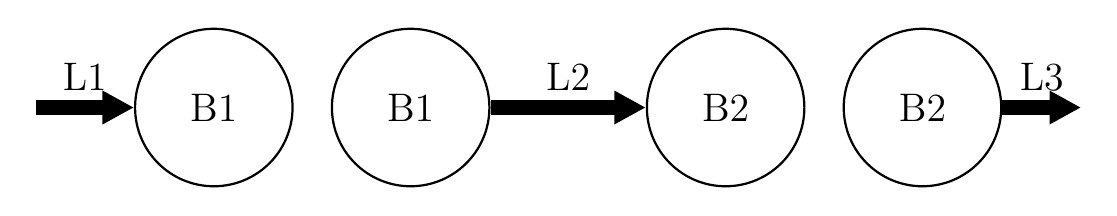
\begin{tikzpicture}[every node/.style={font=\Large}]
        \draw (0, 0) pic (t1) {Task={B1}};
        \draw (2.5, 0) pic (t2) {Task={B1}};
        \draw (6.5, 0) pic (t3) {Task={B2}};
        \draw (9,0) pic (t4) {Task={B2}};
        \begin{scope}[line width = \lw, >={Triangle[width=4mm,length=4mm]}, ->]
            \draw ([xshift=-1.25cm] t1-edge.west) -- node[midway, anchor=south]{L1} (t1-edge.west);
            \draw (t2-edge.east) -- node[midway, anchor=south]{L2}  (t3-edge.west);
            \draw[line width = \lw, ->] (t4-edge.east) -- node[midway, anchor=south]{L3} ([xshift=1cm] t4-edge.east);
        \end{scope}
    \end{tikzpicture}
\end{document}
